% Created by tikzDevice version 0.7.0 on 2014-11-19 19:56:33
% !TEX encoding = UTF-8 Unicode
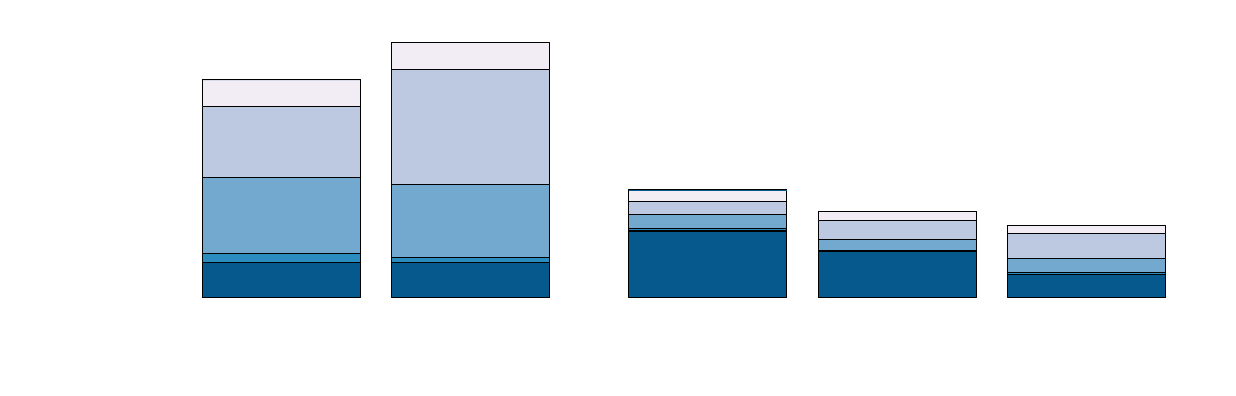
\begin{tikzpicture}[x=1pt,y=1pt]
\definecolor[named]{fillColor}{rgb}{1.00,1.00,1.00}
\path[use as bounding box,fill=fillColor,fill opacity=0.00] (0,0) rectangle (426.39,122.86);
\begin{scope}
\path[clip] (  0.00,  0.00) rectangle (426.39,122.86);
\definecolor[named]{drawColor}{rgb}{0.00,0.00,0.00}
\definecolor[named]{fillColor}{rgb}{0.02,0.35,0.55}

\path[draw=drawColor,line width= 0.4pt,line join=round,line cap=round,fill=fillColor] ( 63.13, 25.20) rectangle (120.20, 38.16);
\definecolor[named]{fillColor}{rgb}{0.17,0.55,0.75}

\path[draw=drawColor,line width= 0.4pt,line join=round,line cap=round,fill=fillColor] ( 63.13, 38.16) rectangle (120.20, 41.40);
\definecolor[named]{fillColor}{rgb}{0.45,0.66,0.81}

\path[draw=drawColor,line width= 0.4pt,line join=round,line cap=round,fill=fillColor] ( 63.13, 41.40) rectangle (120.20, 68.87);
\definecolor[named]{fillColor}{rgb}{0.74,0.79,0.88}

\path[draw=drawColor,line width= 0.4pt,line join=round,line cap=round,fill=fillColor] ( 63.13, 68.87) rectangle (120.20, 94.24);
\definecolor[named]{fillColor}{rgb}{0.95,0.93,0.96}

\path[draw=drawColor,line width= 0.4pt,line join=round,line cap=round,fill=fillColor] ( 63.13, 94.24) rectangle (120.20,104.09);
\definecolor[named]{fillColor}{rgb}{0.02,0.35,0.55}

\path[draw=drawColor,line width= 0.4pt,line join=round,line cap=round,fill=fillColor] ( 63.13,104.09) rectangle (120.20,104.09);

\path[draw=drawColor,line width= 0.4pt,line join=round,line cap=round,fill=fillColor] (131.61, 25.20) rectangle (188.68, 37.99);
\definecolor[named]{fillColor}{rgb}{0.17,0.55,0.75}

\path[draw=drawColor,line width= 0.4pt,line join=round,line cap=round,fill=fillColor] (131.61, 37.99) rectangle (188.68, 39.72);
\definecolor[named]{fillColor}{rgb}{0.45,0.66,0.81}

\path[draw=drawColor,line width= 0.4pt,line join=round,line cap=round,fill=fillColor] (131.61, 39.72) rectangle (188.68, 66.07);
\definecolor[named]{fillColor}{rgb}{0.74,0.79,0.88}

\path[draw=drawColor,line width= 0.4pt,line join=round,line cap=round,fill=fillColor] (131.61, 66.07) rectangle (188.68,107.62);
\definecolor[named]{fillColor}{rgb}{0.95,0.93,0.96}

\path[draw=drawColor,line width= 0.4pt,line join=round,line cap=round,fill=fillColor] (131.61,107.62) rectangle (188.68,117.51);
\definecolor[named]{fillColor}{rgb}{0.02,0.35,0.55}

\path[draw=drawColor,line width= 0.4pt,line join=round,line cap=round,fill=fillColor] (131.61,117.51) rectangle (188.68,117.53);

\path[draw=drawColor,line width= 0.4pt,line join=round,line cap=round,fill=fillColor] (217.22, 25.20) rectangle (274.29, 49.37);
\definecolor[named]{fillColor}{rgb}{0.17,0.55,0.75}

\path[draw=drawColor,line width= 0.4pt,line join=round,line cap=round,fill=fillColor] (217.22, 49.37) rectangle (274.29, 50.35);
\definecolor[named]{fillColor}{rgb}{0.45,0.66,0.81}

\path[draw=drawColor,line width= 0.4pt,line join=round,line cap=round,fill=fillColor] (217.22, 50.35) rectangle (274.29, 55.37);
\definecolor[named]{fillColor}{rgb}{0.74,0.79,0.88}

\path[draw=drawColor,line width= 0.4pt,line join=round,line cap=round,fill=fillColor] (217.22, 55.37) rectangle (274.29, 60.17);
\definecolor[named]{fillColor}{rgb}{0.95,0.93,0.96}

\path[draw=drawColor,line width= 0.4pt,line join=round,line cap=round,fill=fillColor] (217.22, 60.17) rectangle (274.29, 64.31);
\definecolor[named]{fillColor}{rgb}{0.02,0.35,0.55}

\path[draw=drawColor,line width= 0.4pt,line join=round,line cap=round,fill=fillColor] (217.22, 64.31) rectangle (274.29, 64.32);

\path[draw=drawColor,line width= 0.4pt,line join=round,line cap=round,fill=fillColor] (285.71, 25.20) rectangle (342.78, 41.89);
\definecolor[named]{fillColor}{rgb}{0.17,0.55,0.75}

\path[draw=drawColor,line width= 0.4pt,line join=round,line cap=round,fill=fillColor] (285.71, 41.89) rectangle (342.78, 42.38);
\definecolor[named]{fillColor}{rgb}{0.45,0.66,0.81}

\path[draw=drawColor,line width= 0.4pt,line join=round,line cap=round,fill=fillColor] (285.71, 42.38) rectangle (342.78, 46.44);
\definecolor[named]{fillColor}{rgb}{0.74,0.79,0.88}

\path[draw=drawColor,line width= 0.4pt,line join=round,line cap=round,fill=fillColor] (285.71, 46.44) rectangle (342.78, 53.04);
\definecolor[named]{fillColor}{rgb}{0.95,0.93,0.96}

\path[draw=drawColor,line width= 0.4pt,line join=round,line cap=round,fill=fillColor] (285.71, 53.04) rectangle (342.78, 56.46);
\definecolor[named]{fillColor}{rgb}{0.02,0.35,0.55}

\path[draw=drawColor,line width= 0.4pt,line join=round,line cap=round,fill=fillColor] (285.71, 56.46) rectangle (342.78, 56.50);

\path[draw=drawColor,line width= 0.4pt,line join=round,line cap=round,fill=fillColor] (354.19, 25.20) rectangle (411.27, 33.70);
\definecolor[named]{fillColor}{rgb}{0.17,0.55,0.75}

\path[draw=drawColor,line width= 0.4pt,line join=round,line cap=round,fill=fillColor] (354.19, 33.70) rectangle (411.27, 34.32);
\definecolor[named]{fillColor}{rgb}{0.45,0.66,0.81}

\path[draw=drawColor,line width= 0.4pt,line join=round,line cap=round,fill=fillColor] (354.19, 34.32) rectangle (411.27, 39.35);
\definecolor[named]{fillColor}{rgb}{0.74,0.79,0.88}

\path[draw=drawColor,line width= 0.4pt,line join=round,line cap=round,fill=fillColor] (354.19, 39.35) rectangle (411.27, 48.47);
\definecolor[named]{fillColor}{rgb}{0.95,0.93,0.96}

\path[draw=drawColor,line width= 0.4pt,line join=round,line cap=round,fill=fillColor] (354.19, 48.47) rectangle (411.27, 51.50);
\definecolor[named]{fillColor}{rgb}{0.02,0.35,0.55}

\path[draw=drawColor,line width= 0.4pt,line join=round,line cap=round,fill=fillColor] (354.19, 51.50) rectangle (411.27, 51.52);
\end{scope}
\end{tikzpicture}
